% 1988 年全国卷理科第 9 题：正四棱台
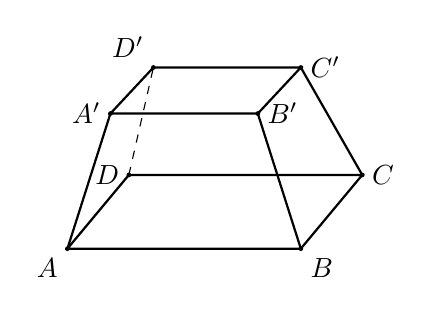
\begin{tikzpicture}[scale=0.78,>=stealth]
  \coordinate (A) at (0,0);
  \coordinate (B) at (3.8,0);
  \coordinate (C) at (4.8,1.2);
  \coordinate (D) at (1.0,1.2);
  \coordinate (Ap) at (0.7,2.2);
  \coordinate (Bp) at (3.1,2.2);
  \coordinate (Cp) at (3.8,2.95);
  \coordinate (Dp) at (1.4,2.95);
  \draw[thick] (A)--(B)--(C)--(D)--cycle;
  \draw[thick] (Ap)--(Bp)--(Cp)--(Dp)--cycle;
  \draw[thick] (A)--(Ap) (B)--(Bp) (C)--(Cp);
  \draw[dashed] (D)--(Dp);
  \fill (A) circle (1.1pt) node[below left] {$A$};
  \fill (B) circle (1.1pt) node[below right] {$B$};
  \fill (C) circle (1.1pt) node[right] {$C$};
  \fill (D) circle (1.1pt) node[left] {$D$};
  \fill (Ap) circle (1.1pt) node[left] {$A'$};
  \fill (Bp) circle (1.1pt) node[right] {$B'$};
  \fill (Cp) circle (1.1pt) node[right] {$C'$};
  \fill (Dp) circle (1.1pt) node[above left] {$D'$};
\end{tikzpicture}
